\section{In-context learning performance} \label{sec:icl-performance}

We first investigated how effectively frontier LLMs could generate linguistically grounded mnemonics through in-context learning. This exploration aimed to establish baseline performance and identify optimal prompting strategies before progressing to more resource-intensive approaches.

\subsection{Experimental setup}

We compared different in-context learning approaches using a test set of 50 vocabulary words from SAT, GRE, TOEFL tests, evaluating four distinct prompting strategies with \xteachermodel (multimodal) and \teachermodel (reasoning) \citep{DeepSeek-AIDEEPSEEKR12025,DeepSeekV32025}.

We then designed prompts $p$ and prompted the model $M$ to generate a \lgm \mnem for \vocab. Generally, a prompt $p$ consists of a task description $t$, a vocabulary \vocab, VAM model \Cref{app:mnemonic-characteristics}, and optionally demonstration examples of \lgms $d$. $t$ could be as simple as "Generate a linguistically grounded mnemonic for the word \vocab" (vanilla) or involve several steps\footnote{analyze vocabulary and its linguistic features -> assess which features are the most relevant to learners -> construct a mnemonic based on the selected features and meet other characteristics of good mnemonics}. To elicit reasoning in \xteachermodel, we added the phrase "Let's think step by step" to all the prompts, a common strategy in prompting LLMs for reasoning tasks \citep{weiChainofThoughtPromptingElicits2022}. We repeated this process for 50 vocabulary \vocab, 4 prompts $p$, and 2 models $M$, executing 400 total API requests. Full description of prompts is in \Cref{app:prompt-usage}.

We used \verb|curator| \citep{BespokeLabBESPOKE2025} to standardize API calls, manage rate limits, and handle retries across experiments. We evaluated the outputs based on two criteria: \numlist{1} lingusitic grounding, whether there is at least one of the linguistic features (\Cref{tab:linguistic-features}) and \numlist{2} overall quality, through manual review using the given rubric (\Cref{fig:good-bad-mnemonics}).

\subsection{Results} \label{sec:icl-results}

\begin{figure}[htb]
  \centering
  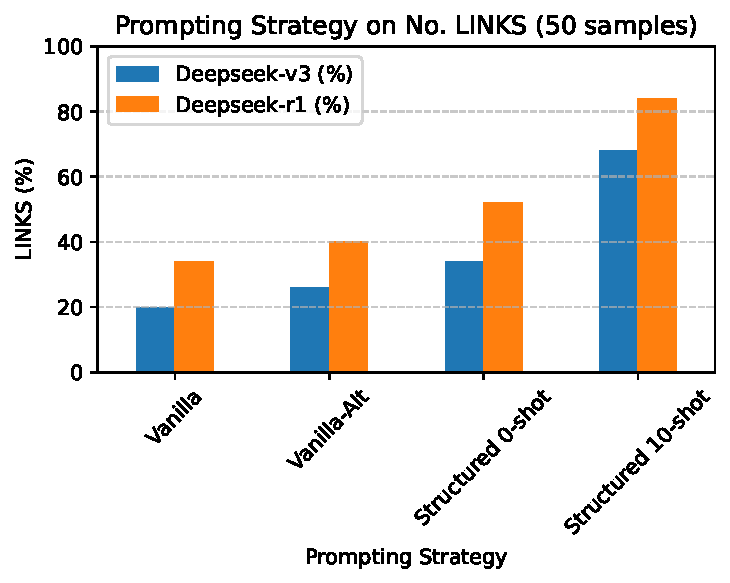
\includegraphics[width=\linewidth]{figures/prompt_comparison.pdf}
  \caption{Comparison of prompting methods (details in \Cref{app:prompt-usage}). Y-axis shows percentage of \lgms generated out of 50 requests sent for 50 vocabulary \vocab for each prompt $p$.}
  \label{fig:prompting-methods}
\end{figure}

As shown in \Cref{fig:prompting-methods}, \teachermodel consistently outperformed \xteachermodel across all prompting strategies, confirming our hypothesis that reasoning models better suit our tasks.

Notably, simply changing terminology from "mnemonic" to "memory cue" increased linguistically grounded responses from 20\% to 26\% for \xteachermodel and from 34\% to 40\% for \teachermodel, suggesting pre-training biases may associate "mnemonic" primarily with acronyms or keyword methods \citep{hackmannWordImportanceExplains2024}.

We also noted \teachermodel tended to generate lengthy, divergent reasoning traces, so we instructed it to stop analysis of linguistic features when it found a good enough mnemonic. Combining this instruction with structured output format and multi-task instructions further improved performance, with \teachermodel achieving 52\% success rate, confirming that shorter reasoning traces can be equally effective \citep{xuChainDraftThinking2025} and that explicit task instructions can enhance performance \citep{yinDidYouRead2023}.

The structured 10-shot CoT prompt, which included examples of linguistic reasoning before mnemonic generation, yielded the highest success rates: 68\% for \xteachermodel and 84\% for \teachermodel. This approach effectively guided models to balance linguistic grounding and memorability.

Our qualitative analysis revealed three key patterns: \numlist{1} LLMs defaulted to surface-level associations rather than deeper linguistic analysis. \numlist{2} Both models favored etymology and morphology in their linguistic analysis, but they usually combined with phonetic or orthographic keywords in generated mnemonics \numlist{3} Several mnemonics are linguistically grounded but not memorable, despite the presence of both requirements in the prompt.

These findings indicated that while LLMs possess substantial linguistic knowledge for English language accessible through appropriate prompting, they benefit from structured guidance to apply this knowledge effectively for mnemonic generation. The superior performance of few-shot reasoning suggested that reasoning elicitation is crucial for high-quality, linguistically grounded mnemonics.

Based on these insights, we selected the 10-shot CoT prompting approach to generate our synthetic dataset for model distillation.
